\documentclass[11pt]{article}

\usepackage[utf8]{inputenc}
\usepackage{pgfplots}
\pgfplotsset{compat=1.18, width=10cm}

\begin{document}

\section{2D Plots}

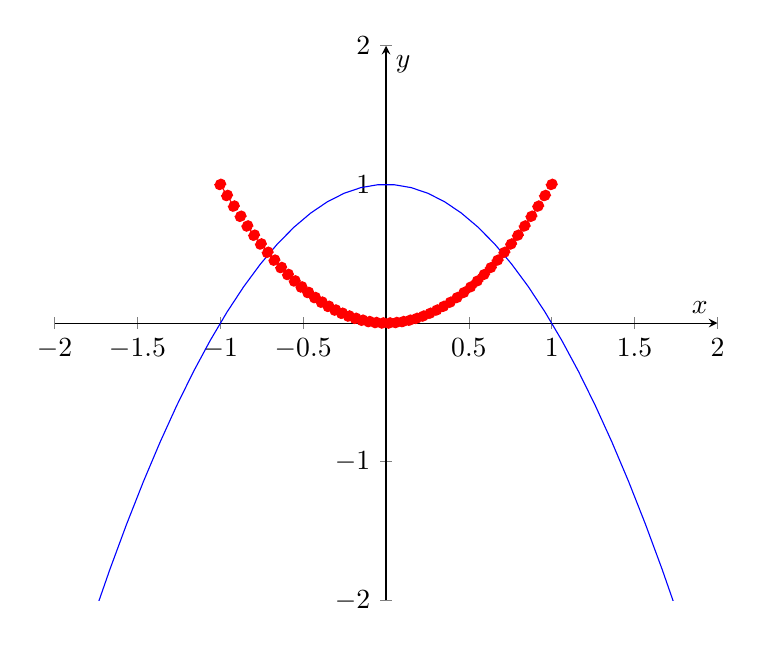
\begin{tikzpicture}
\begin{axis}[xmin=-2, xmax=2, ymin=-2, ymax=2, axis lines=middle, xlabel=$x$, ylabel=$y$]
\addplot[color=red, dashed, mark=*, samples=50, domain=-1:1]{x^2};
\addplot[color=blue, samples=100]{1-x^2};
\end{axis}
\end{tikzpicture}\\[10pt]

\begin{tikzpicture}
    \begin{axis}[clip=false,
        xmin=0, xmax=2.5*pi,
        ymin=-1.5, ymax=1.5,
        axis lines=middle,
        xtick={0, pi/2, pi, 3*pi/2, 2*pi},
        xticklabels={$0$, $\frac{\pi}{2}$, $\pi$, $\frac{3\pi}{2}$, $2\pi$},
        xticklabel style={anchor=south west},
        xmajorgrids=true,
        grid style=dashed,
        ]
        \addplot[domain=0:2*pi,red]{sin(deg(x))}node[right,pos=0.9]{$f(x)=\sin x$};
        \addplot[domain=0:2*pi,,blue]{cos(deg(x))}
        node[right,pos=1]{$f(x)=\cos x$};
    \end{axis}
\end{tikzpicture}

\end{document}